\documentclass[tikz, border=1cm]{standalone}
\usepackage{tikz}
\usetikzlibrary{shapes.geometric, arrows.meta, positioning, fit, calc}

\begin{document}

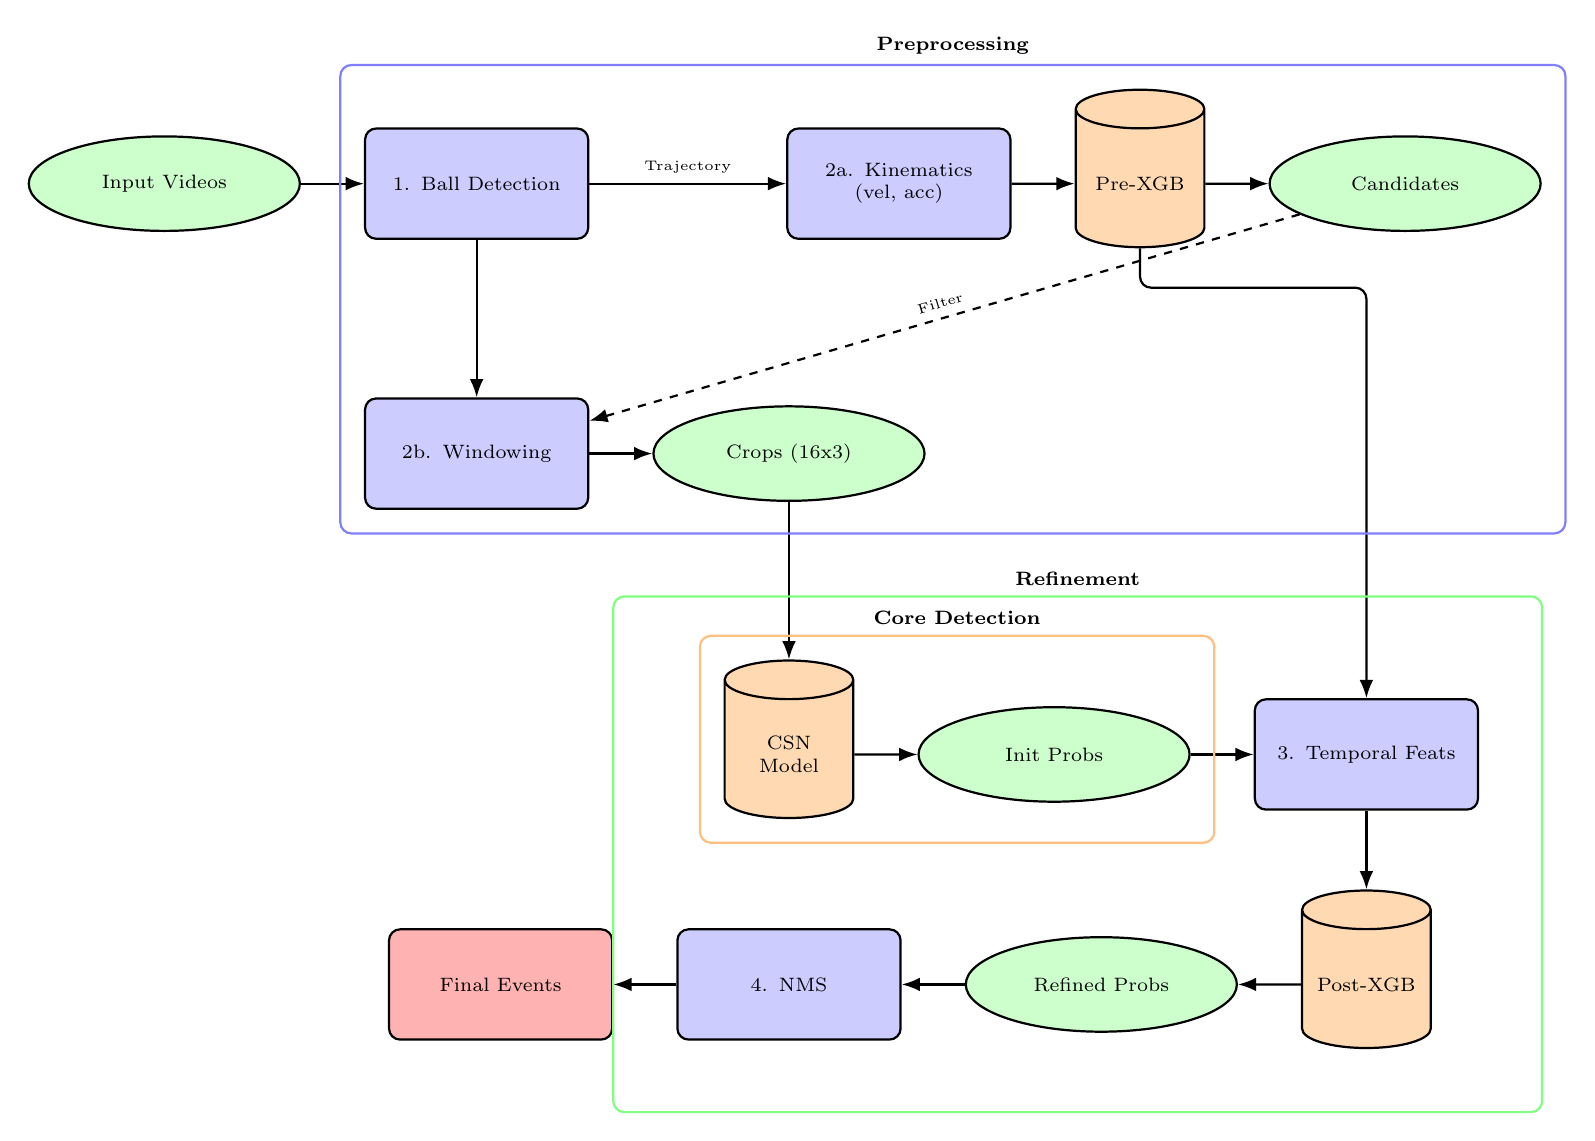
\begin{tikzpicture}[
    node distance=0.8cm and 0.8cm,
    process/.style={rectangle, rounded corners, minimum width=2.8cm, minimum height=1.4cm, text centered, text width=2.6cm, draw=black, fill=blue!20, thick, font=\scriptsize},
    data/.style={ellipse, minimum width=2.5cm, minimum height=1.2cm, text centered, text width=2.2cm, draw=black, fill=green!20, thick, font=\scriptsize},
    model/.style={cylinder, shape border rotate=90, aspect=0.3, minimum height=2.0cm, minimum width=1.5cm, text centered, text width=1.4cm, draw=black, fill=orange!30, thick, font=\scriptsize},
    final/.style={rectangle, rounded corners, minimum width=2.8cm, minimum height=1.4cm, text centered, text width=2.6cm, draw=black, fill=red!30, thick, font=\scriptsize},
    arrow/.style={-Latex, thick},
    dashed_arrow/.style={-Latex, thick, dashed},
    stage_label/.style={font=\bfseries\scriptsize, align=center}
]

% --- Row 1: Top Level (Preprocessing) ---
\node (videos) [data] {Input Videos};
\node (ball_det) [process, right=of videos] {1. Ball Detection};

% Extra space for "Trajectory" label
\node (kinematics) [process, right=2.5cm of ball_det] {2a. Kinematics\\(vel, acc)};
\node (pre_xgb) [model, right=of kinematics] {Pre-XGB};
\node (candidates) [data, right=of pre_xgb] {Candidates};

% --- Row 2: Windowing (Stepped Down) ---
\node (sampling) [process, below=2cm of ball_det] {2b. Windowing};
\node (cnn_input) [data, right=of sampling] {Crops (16x3)};

% --- Row 3: Core Detection (Stepped Down Again) ---
% Increased spacing to 4.5cm to move Core Detection further down
\node (cnn_model) [model, below=2cm of cnn_input] {CSN Model};
\node (cnn_probs) [data, right=of cnn_model] {Init Probs};
\node (temporal_feats) [process, right=of cnn_probs] {3. Temporal Feats};

% --- Row 4: Refinement (Bottom) ---
\node (post_xgb) [model, below=1cm of temporal_feats] {Post-XGB};
\node (final_probs) [data, left=of post_xgb] {Refined Probs};
\node (nms) [process, left=of final_probs] {4. NMS};
\node (output) [final, left=of nms] {Final Events};


% --- Arrows ---

% Row 1
\draw [arrow] (videos) -- (ball_det);
\draw [arrow] (ball_det) -- node[midway, above, font=\tiny] {Trajectory} (kinematics);
\draw [arrow] (kinematics) -- (pre_xgb);
\draw [arrow] (pre_xgb) -- (candidates);

% Row 1 -> Row 2
\draw [arrow] (ball_det) -- (sampling);
\draw [dashed_arrow] (candidates) -- node[midway, above, sloped, font=\tiny] {Filter} (sampling);

% Row 2 -> Row 3
\draw [arrow] (sampling) -- (cnn_input);
\draw [arrow] (cnn_input) -- (cnn_model); % Down step
\draw [arrow] (cnn_model) -- (cnn_probs);
\draw [arrow] (cnn_probs) -- (temporal_feats);

% Pre-XGB -> Temporal Feats (Long connection)
% Route: From Pre-XGB (Row 1) to Temporal Feats (Row 3)
\draw [arrow, rounded corners] (pre_xgb.south) -- ++(0,-0.5) -| (temporal_feats.north);


% Row 3 -> Row 4
\draw [arrow] (temporal_feats) -- (post_xgb);
\draw [arrow] (post_xgb) -- (final_probs);
\draw [arrow] (final_probs) -- (nms);
\draw [arrow] (nms) -- (output);


% --- Bounding Boxes ---
\node[draw=blue!50, thick, rounded corners, inner sep=0.3cm, fit=(ball_det) (kinematics) (pre_xgb) (candidates) (sampling), label={[stage_label]above:Preprocessing}] {};

% Core Detection (Inner Box)
\node[draw=orange!50, thick, rounded corners, inner sep=0.3cm, fit=(cnn_model) (cnn_probs), label={[stage_label]above:Core Detection}] {};

% Refinement (Outer Box - Enclosing Core Detection)
% Includes Core Detection nodes + Refinement nodes
\node[draw=green!50, thick, rounded corners, inner sep=0.8cm, fit=(cnn_model) (cnn_probs) (temporal_feats) (post_xgb) (nms), label={[stage_label]above:Refinement}] {};

\end{tikzpicture}

\end{document}
